\documentclass{beamer}
\usepackage{../tut-slides}
\usepackage{../mathoperatorsAuD}

\usepackage{amsmath,amssymb}
\usepackage{bm}
\usepackage{csquotes}
\usepackage{enumerate}
%\usepackage[inline]{enumitem} 		%customize label
%\newcommand{\labelitemi}{\raisebox{1pt}{\scalebox{.9}{$\blacktriangleright$}}}
%\newcommand{\labelitemii}{$\vartriangleright$}
%\newcommand{\labelitemiii}{--}
\setbeamertemplate{itemize item}{\raisebox{1pt}{\scalebox{.9}{$\blacktriangleright$}}}
\setbeamertemplate{itemize subitem}{$\vartriangleright$}

\usepackage{booktabs}
\usepackage{tabularx}
\usepackage{tabu}
\newcommand*\head{\rowfont{\bfseries}}
\newcommand*{\tw}{\rowfont{\ttfamily}}
\renewcommand{\tabularxcolumn}[1]{>{\hspace{0pt}}m{#1}}

\usepackage{cancel}

%%%% FARBEN %%%%%
\newcommand{\orange}[1]{\textcolor{cdorange}{#1}}
\newcommand{\green}[1]{\textcolor{cdgreen}{#1}}
\newcommand{\purple}[1]{\textcolor{cdpurple}{#1}}


%%%% EBNF-Terme %%%%
\usepackage{../syntaxdiagrammEBNF}

\begin{document}	
	\title{Algorithmen und Datenstrukturen}
	\subtitle{Übung 2: Syntaxdiagramme \& EBNF}
	\author{Eric Kunze}
	\email{eric.kunze@tu-dresden.de}
	\city{TU Dresden}
%	\institute{Lehrstuhl für Grundlagen der Programmierung}
	\titlegraphic{
\includegraphics[width=2cm]{../TUD-white.pdf}}
	\date{06.11.2020}

	\maketitle


%%%%%%%%%%%%%%%%%%%%%%%%%%%%%%%%%%%%%%%%%%%%%%%%%%%%%%%%%%%%%%%%%%%%%%%%%%%%%

\begin{frame} \frametitle{Videoempfehlung}
	
	
	Prof. Dr. Markus Krötzsch hat im vergangenen Wintersemester 2020/21 die Vorlesung \enquote{Formale Systeme} (3. Semester) in Form von YouTube-Videos gehalten. Diese Vorlesung beschäftigt sich vertieft mit formalen Sprachen.
	
	Die Einleitung entspricht ungefähr dem Inhalt der ersten Übung:
	\begin{itemize}
		\item  \url{https://youtu.be/Lma6jaPnD-I}
	\end{itemize}
\end{frame}

\section{Syntaxdiagramme}

\begin{frame} \frametitle{Syntaxdiagramme}
	\small
	Beispiel eines Syntaxdiagrammsystems mit Startdiagramm $S$:
	\begin{center}
		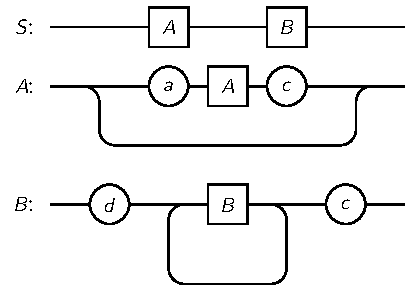
\includegraphics[width=.5\textwidth]{tut02_syntax-dia-bsp.pdf}
	\end{center}
	\begin{itemize}
		\item[] \scalebox{0.6}{\tikz{\node [rectangle, draw, thick] {A};}} $\dots$
		Nichtterminalsymbol = syntaktische Variable
		\item[] \scalebox{0.5}{\tikz{\node [circle, draw, thick] {a};}} $\dots$
		Terminalsymbol
	\end{itemize}
\end{frame}

\begin{frame} \frametitle{Rücksprungalgorithmus}
	\small
	\textbf{Rücksprungalgorithmus}
	\begin{itemize}
		\item Ziel: Nachweis von Zugehörigkeit eines Wortes zu einer Sprache
		\item jedes Kästchen bekommt eindeutige Marke (Rücksprungadresse)
		\item beim Betreten eines Syntaxdiagramms wird eine Marke auf den Keller gelegt
	\end{itemize}

	Hauptaugenmerk: \\
	Protokollierung von Wortentstehung \& Markenkeller
	\begin{itemize}
		\item jede Zeile entspricht dem Aufenthalt in einem Syntaxdiagramm
		\item jede Zeile führt eine Operation auf dem Markenkeller durch
	\end{itemize}
\end{frame}

\begin{frame} \frametitle{Aufgabe 1}
	\small
	
	\begin{minipage}[t]{\dimexpr0.55\linewidth-\fboxrule-\fboxsep}
		Gegeben sei das folgende Syntaxdiagrammsystem $\mathcal{U}$ mit Startdiagramm $S$:
		
		\vspace{2em}
		
		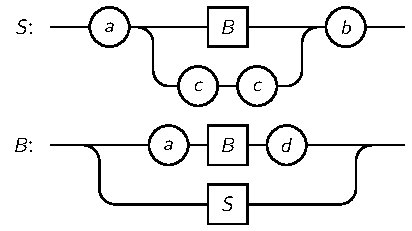
\includegraphics[width=.9\textwidth]{tut02_syntax-dia-1a.pdf}
	\end{minipage}	
	\hspace{1em} \pause
	\begin{minipage}[t]{\dimexpr0.35\linewidth-\fboxrule-\fboxsep}
		Beispiele für Wörter, die das System $\mathcal{U}$ erzeugt:
		
		\begin{itemize}
			\item $\green{a} \ accb \ \green{b}$
			\item $\green{a} \ \green{a} \ accb \ \green{b} \ \green{b}$
		\end{itemize}
	
		\begin{itemize}
			\item $\green{a} \ \purple{a} \ accb \ \purple{d} \ \green{b}$
			\item $\green{a} \ \purple{a} \ \purple{a} \ accb \ \purple{d} \ \purple{d} \ \green{b}$
		\end{itemize}
	
		\begin{itemize}
			\item $\green{a} \ \purple{a} \ \green{a} \ accb \ \green{b} \ \purple{d} \ \green{b}$
		\end{itemize}
	\end{minipage}
\end{frame}

\begin{frame} \frametitle{Aufgabe 1 --- Teil (b)}
	\begin{minipage}{\dimexpr0.5\linewidth-\fboxrule-\fboxsep}
		Wort: \texttt{aaaaccbdbb}
		
		\vspace{2em} \small
		\textbf{Protokollierungszeitpunkte:}
		\begin{itemize}
			\item jeder Aufenthalt in einem Syntaxdiagramm entspricht einer Zeile
			\item jede Zeile führt eine Operation auf dem Markenkeller aus
			\item $\cancel{3}$ = Rücksprung zu Marke $3$
		\end{itemize}
	\end{minipage}
	\pause
	\begin{minipage}{\dimexpr0.5\linewidth-\fboxrule-\fboxsep}
		\centering
		\begin{tabular}{l|r}
			\hline
			Wort & Markenkeller \\ \hline \pause
			a & 1 \\ \pause
			a & 31 \\ \pause
			aa & 131 \\ \pause
			aaa & 2131 \\ \pause
			aaa & 32131 \\ \pause
			aaaaccb & $\cancel{3} 2131$ \\ \pause
			aaaaccb & $\cancel{2}131$ \\ \pause
			aaaaccbd & $\cancel{1}31$ \\ \pause
			aaaaccbdb & $\cancel{3}1$ \\ \pause
			aaaaccbdb & $\cancel{1}$ \\ \pause
			aaaaccbdbb & -- \\ \hline
		\end{tabular}
	\end{minipage}
\end{frame}

\begin{frame} \frametitle{Grundkonstruktion von Syntaxdiagrammen}
	$L = L_A \cdot L_B$
	\vspace{-.5\baselineskip} \pause
	\begin{center}
		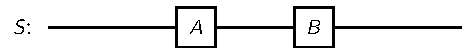
\includegraphics[width=6cm]{tut02_syntax-dia-basic-conc.pdf}
	\end{center}
	\pause

	$L = \menge{a^n \ L_A \ b^n : n \alert{\bm\ge} 0}$
	\vspace{-.5\baselineskip} \pause
	\begin{center}
		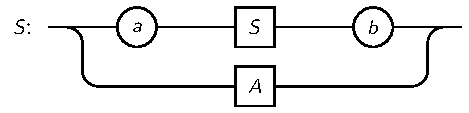
\includegraphics[width=6cm]{tut02_syntax-dia-basic0.pdf}
	\end{center}
	\pause

	$L = \menge{a^n \ L_A \ b^n : n \alert{\bm >} 0}$
	\vspace{-.5\baselineskip} \pause
	\begin{center}
		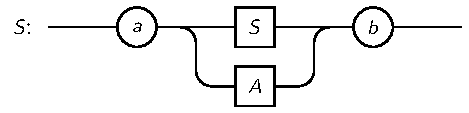
\includegraphics[width=6cm]{tut02_syntax-dia-basic1.pdf}
	\end{center}
	
	\vspace{-\baselineskip} \pause
	kleine Tricks:
	\begin{itemize}
		\item $a^{2n} = (a^2)^n = (aa)^n$
		\item $a^{2n+1} = a \ a^{2n} = a \ (aa)^n$
	\end{itemize}
\end{frame}

\begin{frame} \frametitle{Aufgabe 1 --- Teil (c)}
	\begin{align*}
		L &= \menge{a^{2i} c b^{3i} c^k d^{2k+1} \mid i > 0, k \ge 0} \\
		\onslide<2->{&= \menge{a^{2i} c b^{3i} \mid i > 0} * \menge{c^k d^{2k+1} \mid k \ge 0} \\
		&= \menge{\orange{(aa)^i} c \orange{(bbb)^i} \mid i > 0} * \menge{\purple{c^k} d \purple{(dd)^k}  \mid k \ge 0}}
	\end{align*}
	
	\centering
	\onslide<3->{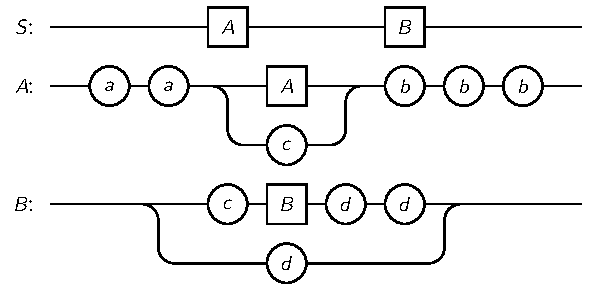
\includegraphics[width=.9\textwidth]{tut02_syntax-dia-1c.pdf}}
\end{frame}


\section{Extended Backus-Naur-Form}

\begin{frame} \frametitle{EBNF-Definition}
	\small
	\begin{itemize}
		\item EBNF-Definition besteht aus endlicher Menge von EBNF-Regeln.
		\item Jede EBNF-Regel besteht aus einer linken und einer rechten Seite, die rechte Seite ist ein EBNF-Term.
	\end{itemize}
	\pause
	\begin{block}{Definition: EBNF-Term}
		Seien $V$ eine endliche Menge (syntaktische Variablen) und $\Sigma$ eine endliche Menge (Terminalsymbole) mit $V \cap \Sigma = \emptyset$. Die Menge der EBNF-Terme über $V$ und $\Sigma$ (notiere: $T(\Sigma, V)$), ist die \emph{kleinste} Menge $T \subseteq \brackets{V \cup \Sigma \cup \menge{\hat{\{}, \hat{\}}, \hat{[}, \hat{]}, \hat{(}, \hat{)}, \hat{|}}}$ mit $V \subseteq T$, $\Sigma \subseteq T$ und
		\begin{itemize}
			\item Wenn $\alpha \in T$, so auch $\rdb{\alpha} \in T$, $\wdh{\alpha} \in T$, $\byp{\alpha} \in T$.
			\item Wenn $\alpha_1, \alpha_2 \in T$, so auch $\opt{\alpha_1}{\alpha_2} \in T$, $\alpha_1 \alpha_2 \in T$
		\end{itemize}
	\end{block}
\end{frame}

\begin{frame} \frametitle{Übersetzung EBNF $\leftrightarrow$ Syntaxdiagramme}
	\small
	Sei $v \in V$ und $w \in \Sigma$. $trans(v) =$ 
	\scalebox{0.7}{
		\tikz[baseline=-0.5ex]{\coordinate (start) at (0,0); \coordinate (end) at (2,0); \nonterminal{v}{$v$}{(1,0)}; \draw[thick] (start) -- (v) -- (end);}
	};
	$trans(w) =$ 
	\scalebox{0.7}{
		\tikz[baseline=-0.5ex]{\coordinate (start) at (0,0); \coordinate (end) at (2,0); \terminal{w}{$w$}{(1,0)}; \draw[thick] (start) -- (w) -- (end);}
	}

	Sei $\alpha \in T(\Sigma, V)$ ein EBNF-Term. 
	\begin{itemize}
		\item \makebox[2cm][l]{$trans(\ \wdh{\alpha} \ )$} $=$  
		\scalebox{0.7}{
			\tikz[baseline=-0.5ex]{
				\coordinate (start) at (0,0); 
				\coordinate (end) at (4,0);
				\coordinate (mid) at (2,0); \terminals{alpha}{$trans(\alpha)$}{(2,-1)}; 
				\draw[thick] (start) 
				-- coordinate[pos=0.3](l-start) (mid)
				-- coordinate[pos=0.7](l-end) (end);
				\loopleft{alpha}{l-start} 
				\loopright{l-end}{alpha}
			}
		}
		%
		\item \makebox[2cm][l]{$trans(\ \byp{\alpha} \ )$} $=$  
		\scalebox{0.7}{
			\tikz[baseline=-0.5ex]{
				\coordinate (start) at (0,0); 
				\coordinate (end) at (4,0);
				\coordinate (lower) at (2,-1); \terminals{alpha}{$trans(\alpha)$}{(2,0)}; 
				\draw[thick] (start) 
				-- coordinate[midway](l-start) (alpha)
				-- coordinate[midway](l-end) (end);
				\altleft{l-start}{lower}
				\altright{lower}{l-end}
			}
		}
		%
		\item $trans(\ \rdb{\alpha} \ ) = trans(\alpha)$
	\end{itemize}

	Seien $\alpha_1, \alpha_2 \in T(\Sigma, V)$ zwei EBNF-Terme. 
	\begin{itemize}
		\item $trans(\ \alpha_1 \alpha_2 \ ) =$  
		\scalebox{0.7}{
			\tikz[baseline=-0.5ex]{
				\coordinate (start) at (0,0); 
				\coordinate (end) at (6,0); \terminals{alpha1}{$trans(\alpha_1)$}{(2,0)}; 
				\terminals{alpha2}{$trans(\alpha_2)$}{(4,0)}; 
				\draw[thick] (start) 
				-- (alpha1)
				-- (alpha2)
				-- (end);
			}
		}
		
		\item $trans(\ \opt{\alpha_1}{\alpha_2} \ ) =$  
		\scalebox{0.7}{
			\tikz[baseline=-0.5ex]{
				\coordinate (start) at (0,0); 
				\coordinate (end) at (4,0); \terminals{alpha1}{$trans(\alpha_1)$}{(2,0)}; 
				\terminals{alpha2}{$trans(\alpha_2)$}{(2,-1)}; 
				\draw[thick] (start) 
				-- coordinate[midway](l-start) (alpha1)
				-- coordinate[midway](l-end) (end);
				\altleft{l-start}{alpha2}
				\altright{alpha2}{l-end}
			}
		}
	\end{itemize}
	
	\tiny Auszug aus dem Foliensatz der Vorlesung
\end{frame}

\begin{frame} \frametitle{Aufgabe 2 --- Teil (a)}
	\small
	EBNF-Definition $\mathcal{E} = (V,\Sigma,S,R)$ mit $\Sigma = \menge{a,b,c,d}$,
	\begin{align*}
		V = \menge{S,A,B} 
		\quad \und \quad
		R = \Big\{ S &::= A \ \wdh{B} , \\ 
				   A &::= aA \  \opt{bc}{d} , \\
				   B &::= \byp{B} \ b 
		    \qquad \Big\}
	\end{align*}

	\pause
	
	\textbf{Übersetzung in ein Syntaxdiagrammsystem:}
	
	\centering
	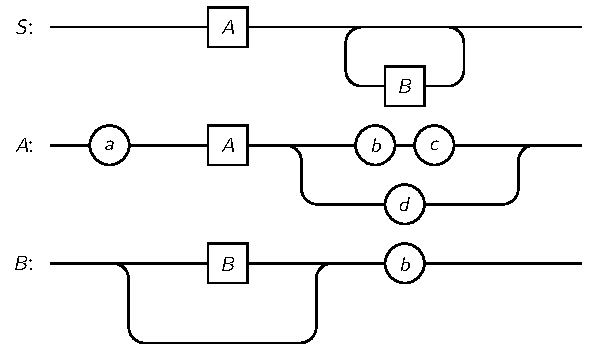
\includegraphics[height=4.5cm]{tut02_syntax-dia-2a.pdf}
\end{frame}

\begin{frame} \frametitle{Aufgabe 2 --- Teil (b)}
	Gegeben sei die Sprache
	\begin{equation*}
		L = \menge{(ab)^n c^{m+1} d^k b^{n+m} : n,m \ge 0, k \ge 1}
	\end{equation*}
	Gesucht ist eine zugehörige EBNF-Definition. \pause
	\begin{equation*}
		L = \menge{\textcolor{cdorange}{(ab)^n} \textcolor{cdpurple}{c^{m+1}} d^k \textcolor{cdpurple}{b^m} \textcolor{cdorange}{b^n} : n,m \ge 0, k \ge 1}
	\end{equation*}
	\pause 
	
	\textbf{EBNF-Definition:} $\mathcal{E} = (V,\Sigma,S,R)$ mit $\Sigma = \menge{a,b,c,d}$, 
	\begin{align*}
		V = \menge{S,A} \quad \und \quad
		R = \Big\{ 
			S &::= \opt{abSb}{A}, \\
			A &::= \opt{cAb}{cd \ \wdh{d}} \enskip 
		\Big\}
	\end{align*}
\end{frame}

\end{document}